% Options for packages loaded elsewhere
\PassOptionsToPackage{unicode}{hyperref}
\PassOptionsToPackage{hyphens}{url}
%
\documentclass[
  ,man]{apa6}
\usepackage{amsmath,amssymb}
\usepackage{lmodern}
\usepackage{iftex}
\ifPDFTeX
  \usepackage[T1]{fontenc}
  \usepackage[utf8]{inputenc}
  \usepackage{textcomp} % provide euro and other symbols
\else % if luatex or xetex
  \usepackage{unicode-math}
  \defaultfontfeatures{Scale=MatchLowercase}
  \defaultfontfeatures[\rmfamily]{Ligatures=TeX,Scale=1}
\fi
% Use upquote if available, for straight quotes in verbatim environments
\IfFileExists{upquote.sty}{\usepackage{upquote}}{}
\IfFileExists{microtype.sty}{% use microtype if available
  \usepackage[]{microtype}
  \UseMicrotypeSet[protrusion]{basicmath} % disable protrusion for tt fonts
}{}
\makeatletter
\@ifundefined{KOMAClassName}{% if non-KOMA class
  \IfFileExists{parskip.sty}{%
    \usepackage{parskip}
  }{% else
    \setlength{\parindent}{0pt}
    \setlength{\parskip}{6pt plus 2pt minus 1pt}}
}{% if KOMA class
  \KOMAoptions{parskip=half}}
\makeatother
\usepackage{xcolor}
\usepackage{graphicx}
\makeatletter
\def\maxwidth{\ifdim\Gin@nat@width>\linewidth\linewidth\else\Gin@nat@width\fi}
\def\maxheight{\ifdim\Gin@nat@height>\textheight\textheight\else\Gin@nat@height\fi}
\makeatother
% Scale images if necessary, so that they will not overflow the page
% margins by default, and it is still possible to overwrite the defaults
% using explicit options in \includegraphics[width, height, ...]{}
\setkeys{Gin}{width=\maxwidth,height=\maxheight,keepaspectratio}
% Set default figure placement to htbp
\makeatletter
\def\fps@figure{htbp}
\makeatother
\setlength{\emergencystretch}{3em} % prevent overfull lines
\providecommand{\tightlist}{%
  \setlength{\itemsep}{0pt}\setlength{\parskip}{0pt}}
\setcounter{secnumdepth}{-\maxdimen} % remove section numbering
% Make \paragraph and \subparagraph free-standing
\ifx\paragraph\undefined\else
  \let\oldparagraph\paragraph
  \renewcommand{\paragraph}[1]{\oldparagraph{#1}\mbox{}}
\fi
\ifx\subparagraph\undefined\else
  \let\oldsubparagraph\subparagraph
  \renewcommand{\subparagraph}[1]{\oldsubparagraph{#1}\mbox{}}
\fi
\newlength{\cslhangindent}
\setlength{\cslhangindent}{1.5em}
\newlength{\csllabelwidth}
\setlength{\csllabelwidth}{3em}
\newlength{\cslentryspacingunit} % times entry-spacing
\setlength{\cslentryspacingunit}{\parskip}
\newenvironment{CSLReferences}[2] % #1 hanging-ident, #2 entry spacing
 {% don't indent paragraphs
  \setlength{\parindent}{0pt}
  % turn on hanging indent if param 1 is 1
  \ifodd #1
  \let\oldpar\par
  \def\par{\hangindent=\cslhangindent\oldpar}
  \fi
  % set entry spacing
  \setlength{\parskip}{#2\cslentryspacingunit}
 }%
 {}
\usepackage{calc}
\newcommand{\CSLBlock}[1]{#1\hfill\break}
\newcommand{\CSLLeftMargin}[1]{\parbox[t]{\csllabelwidth}{#1}}
\newcommand{\CSLRightInline}[1]{\parbox[t]{\linewidth - \csllabelwidth}{#1}\break}
\newcommand{\CSLIndent}[1]{\hspace{\cslhangindent}#1}
\ifLuaTeX
\usepackage[bidi=basic]{babel}
\else
\usepackage[bidi=default]{babel}
\fi
\babelprovide[main,import]{english}
% get rid of language-specific shorthands (see #6817):
\let\LanguageShortHands\languageshorthands
\def\languageshorthands#1{}
% Manuscript styling
\usepackage{upgreek}
\captionsetup{font=singlespacing,justification=justified}

% Table formatting
\usepackage{longtable}
\usepackage{lscape}
% \usepackage[counterclockwise]{rotating}   % Landscape page setup for large tables
\usepackage{multirow}		% Table styling
\usepackage{tabularx}		% Control Column width
\usepackage[flushleft]{threeparttable}	% Allows for three part tables with a specified notes section
\usepackage{threeparttablex}            % Lets threeparttable work with longtable

% Create new environments so endfloat can handle them
% \newenvironment{ltable}
%   {\begin{landscape}\centering\begin{threeparttable}}
%   {\end{threeparttable}\end{landscape}}
\newenvironment{lltable}{\begin{landscape}\centering\begin{ThreePartTable}}{\end{ThreePartTable}\end{landscape}}

% Enables adjusting longtable caption width to table width
% Solution found at http://golatex.de/longtable-mit-caption-so-breit-wie-die-tabelle-t15767.html
\makeatletter
\newcommand\LastLTentrywidth{1em}
\newlength\longtablewidth
\setlength{\longtablewidth}{1in}
\newcommand{\getlongtablewidth}{\begingroup \ifcsname LT@\roman{LT@tables}\endcsname \global\longtablewidth=0pt \renewcommand{\LT@entry}[2]{\global\advance\longtablewidth by ##2\relax\gdef\LastLTentrywidth{##2}}\@nameuse{LT@\roman{LT@tables}} \fi \endgroup}

% \setlength{\parindent}{0.5in}
% \setlength{\parskip}{0pt plus 0pt minus 0pt}

% Overwrite redefinition of paragraph and subparagraph by the default LaTeX template
% See https://github.com/crsh/papaja/issues/292
\makeatletter
\renewcommand{\paragraph}{\@startsection{paragraph}{4}{\parindent}%
  {0\baselineskip \@plus 0.2ex \@minus 0.2ex}%
  {-1em}%
  {\normalfont\normalsize\bfseries\itshape\typesectitle}}

\renewcommand{\subparagraph}[1]{\@startsection{subparagraph}{5}{1em}%
  {0\baselineskip \@plus 0.2ex \@minus 0.2ex}%
  {-\z@\relax}%
  {\normalfont\normalsize\itshape\hspace{\parindent}{#1}\textit{\addperi}}{\relax}}
\makeatother

% \usepackage{etoolbox}
\makeatletter
\patchcmd{\HyOrg@maketitle}
  {\section{\normalfont\normalsize\abstractname}}
  {\section*{\normalfont\normalsize\abstractname}}
  {}{\typeout{Failed to patch abstract.}}
\patchcmd{\HyOrg@maketitle}
  {\section{\protect\normalfont{\@title}}}
  {\section*{\protect\normalfont{\@title}}}
  {}{\typeout{Failed to patch title.}}
\makeatother

\usepackage{xpatch}
\makeatletter
\xapptocmd\appendix
  {\xapptocmd\section
    {\addcontentsline{toc}{section}{\appendixname\ifoneappendix\else~\theappendix\fi\\: #1}}
    {}{\InnerPatchFailed}%
  }
{}{\PatchFailed}
\keywords{individual differences, reliability, cognitive control, cognitive abilities, hierarchical models}
\DeclareDelayedFloatFlavor{ThreePartTable}{table}
\DeclareDelayedFloatFlavor{lltable}{table}
\DeclareDelayedFloatFlavor*{longtable}{table}
\makeatletter
\renewcommand{\efloat@iwrite}[1]{\immediate\expandafter\protected@write\csname efloat@post#1\endcsname{}}
\makeatother
\usepackage{csquotes}
\usepackage{bm}
\usepackage{pcl}
\usepackage{amsmath}
\usepackage{setspace}
\ifLuaTeX
  \usepackage{selnolig}  % disable illegal ligatures
\fi
\IfFileExists{bookmark.sty}{\usepackage{bookmark}}{\usepackage{hyperref}}
\IfFileExists{xurl.sty}{\usepackage{xurl}}{} % add URL line breaks if available
\urlstyle{same} % disable monospaced font for URLs
\hypersetup{
  pdftitle={Hierarchical-Model Insights For Planning and Interpreting Individidual-Difference Studies of Cognitive Abilities},
  pdfauthor={Jeffrey N. Rouder1 \& Mahbod Mehrvarz1},
  pdflang={en-EN},
  pdfkeywords={individual differences, reliability, cognitive control, cognitive abilities, hierarchical models},
  hidelinks,
  pdfcreator={LaTeX via pandoc}}

\title{Hierarchical-Model Insights For Planning and Interpreting Individidual-Difference Studies of Cognitive Abilities}
\author{Jeffrey N. Rouder\textsuperscript{1} \& Mahbod Mehrvarz\textsuperscript{1}}
\date{}


\shorttitle{Hierarchical-Model Insights}

\authornote{

Version 2, February, 2023.

Author Contributions: JNR wrote the paper, analyzed the Stroop and flanker effect data, and provided the mathematical derivations. MM analyzed the visual illusion data and overall speed measures. Both authors jointly edited the paper.

Open Science Practices: All data, analyses, and code for drawing the figures and typesetting the table are available at github.com/specl/ctx-reliability.

JNR was supported by NSF 2126976.

Correspondence concerning this article should be addressed to Jeffrey N. Rouder, Department of Cognitive Science, University of California, Irvine, CA, 92697. E-mail: \href{mailto:jrouder@uci.edu}{\nolinkurl{jrouder@uci.edu}}

}

\affiliation{\vspace{0.5cm}\textsuperscript{1} University of California, Irvine}

\abstract{%
Although individual-difference studies have been invaluable in several domains of psychology, there has been less success in cognitive domains using experimental tasks. The problem is often called one of reliability---individual differences in cognitive tasks, especially cognitive-control tasks, seem too unreliable (e.g., Enkavi, et al., PNAS, 2019). In this paper, we use the language of hierarchical models to define a novel reliability measure---a signal-to-noise ratio---that reflects the nature of tasks alone without recourse to sample sizes. Signal-to-noise reliability may be used to plan appropriately powered studies as well as understand the cause of low correlations across tasks should they occur. Although signal-to-noise reliability is motivated by hierarchical models, it may be estimated from a simple calculation using straightforward summary statistics.
}



\begin{document}
\maketitle

It is popular to study individual differences in cognitive tasks. By understanding how individuals' performance covaries across these tasks, it is perhaps possible to recover an underlying structure. The classic example in cognitive control comes from Miyake et al. (2000), who used latent-variable models to decompose individual differences in cognitive-control tasks into three factors (inhibition, shifting, updating). In the individual-differences approach, participants complete a battery of tasks such as the Stroop task (Stroop, 1935), the flanker task (Eriksen \& Eriksen, 1974), and the antisaccade task (Kane, Bleckley, Conway, \& Engle, 2001) among many others. On each of these tasks, a task score is computed per individual. The matrix of scores per individual across the tasks serves as input (see Figure \ref{fig:usual}) to structural-equation modeling where the covariation across tasks is decomposed into latent variables (Bollen, 1989; Skrondal \& Rabe-Hesketh, 2004). The relations among these latent variables purportedly reveal the underlying structure of cognitive processes.

\begin{figure}
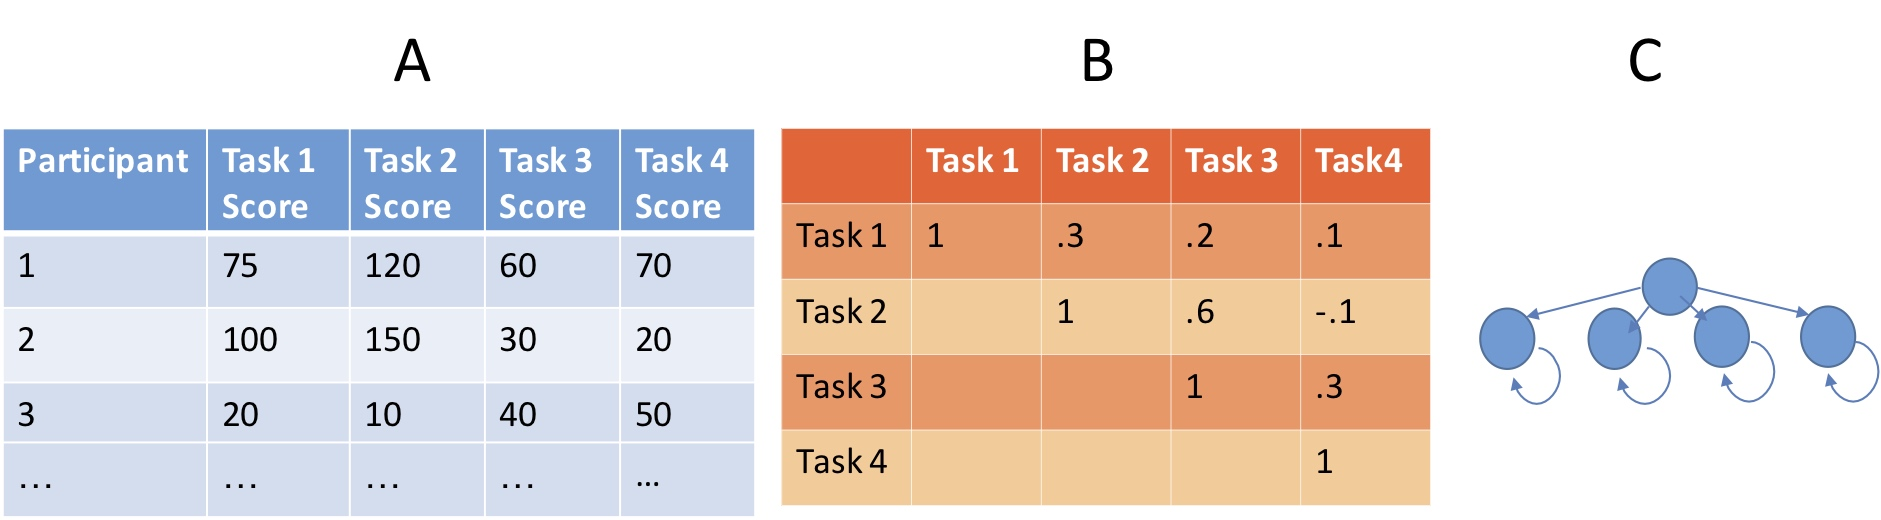
\includegraphics[width=5in]{dataAnalysis} \caption{Usual analysis: The raw data are used to tabulated into individual scores (A). The covariation among these individual scores may be computed (B).  These covariances are decomposed with structural equation models (C).}\label{fig:usual}
\end{figure}

The results using this approach in cognition have been less than stellar, and there is substantial disagreement about the factor structure of cognitive control, attention, and working memory (cf., Rey-Mermet, Gade, and Oberauer (2018), Schubert, Hagemann, and Frischkorn (2017)). Perhaps these disagreements reflect a statistical concern---called here the \emph{reliability crisis}---that cognitive tasks may not be sufficiently reliable to perform latent-variable modeling (Enkavi et al., 2019; Hedge, Powell, \& Sumner, 2018). If tasks have low reliability, then correlations are attenuated, and it is difficult to extract the underlying latent structure of covariation. There are two signatures to the reliability crisis: First, in the domain of cognitive control, several tasks that purportedly measure the same construct do not correlate well. For example, the correlation between flanker and Stroop effects in large studies is often near .1 and rarely greater than .25 (Enkavi et al., 2019; Rey-Mermet et al., 2018; Rouder, Haaf, \& Kumar, in preparation). These results indicate that even if these tasks are truly correlated, the correlation may be so attenuated by low reliability as to not be recoverable. Second, latent-variable decomposition in cognitive-control domains seems unreplicable. This lack of replicability is showcased by Karr et al. (2018) who showed that latent-variable analysis with simulated data infrequently recovered the generating model when the sample sizes and parameter values used in the simulation came from extant studies.

One proposed solution to the reliability crisis is to use hierarchical models to appropriately partition variability into distinct strata (Haines et al., 2020; Matzke et al., 2017; Rouder \& Haaf, 2019). Perhaps by modeling variability and covariability due to trials, conditions, tasks, and people, researchers can improve their recovery of correlations across tasks even in low-reliability environments. Indeed, there is good news on this front---hierarchical models outperform their nonhierarchical competitors and, perhaps more importantly, provide reasonable estimates of uncertainty (Rouder et al., in preparation).

We show here that the \emph{language} of hierarchical models, along with a few quick calculations, can provide a valuable tool in planning and interpreting individual-difference studies. In many ways, our goal is similar to Spearman (1904), who used the language of hierarchical models to develop his famous formula for disattenuating correlations. Our contribution is an update on Spearman's with new features specific for behavioral experiments.

To see the need for a hierarchical-model language, we need look no further than the concept of \emph{reliability}. Suppose two labs are studying the test-retest reliability of a Stroop task, and everything is the same except that one lab runs 200 trials per person per condition and the other only 20 trials per person per condition. The procedure in the second lab yields a much lower test-retest reliability than the first. Hence, the reliability coefficient is not a property of the task itself. It is not helpful to make statements such as ``The Stroop task has low reliability,'' because reliability is critically intertwined with the number of trials per person per condition (henceforth called \emph{trial size}).

Is the reliability crisis merely a crisis of trial size? Is there a measure of reliability that reflects the properties of the task without reference to trial size, and if so, what is it? What is the relationship between trial size, a trial-size invariant measure of reliability and the ability to localize correlations? Hierarchical models provide clear insights into these questions. These insights may be leveraged in planning experiments and interpreting results even if hierarchical models are \emph{not} used in analysis.

\hypertarget{reliability-as-signal-to-noise-ratios}{%
\section{Reliability as Signal-To-Noise Ratios}\label{reliability-as-signal-to-noise-ratios}}

To answer the above questions, we start with a simple hierarchical model of trial noise in a task. Suppose \(I\) people each run \(L\) trials in congruent and incongruent conditions. Let \(i\) denote people, \(k\) denote conditions, and \(\ell\) denote replicate trials. Response times denoted \(Y_{ik\ell}\) are modeled as \(Y_{ik\ell} = \alpha_i +x_k\theta_i+\epsilon_{ik\ell}\), where \(x_k\) contrast codes condition and is -1/2 and 1/2 for congruent and incongruent conditions respectively. Parameter \(\alpha_i\) is the true overall speed of the \(i\)th participant. Parameter \(\theta_i\) is the true difference between incongruent and congruent conditions---it is the \(i\)th participant's true Stroop effect and the main target of analysis. The error term is \(\epsilon_{ik\ell} \sim \mbox{Normal}(0,\sigma^2)\), with \(\sigma^2\) describing the variability of trial noise. The remaining critical specification is on \(\theta_i\), the true Stroop effect for the \(i\)th person. Because each \(\theta_i\) describes a latent attribute of a person, it is reasonable to treat it as random effect: \(\theta_i \sim \mbox{Normal}(\nu,\delta^2)\), where \(\nu\) and \(\delta^2\) describe the population mean and variance. This last step makes the model hierarchical as variability across trials (\(\sigma^2\)) and across people (\(\delta^2\)) are modeled separately.

The usual course is to tabulate a Stroop effect for each person from condition means \(d_i=\bar{Y}_{i2}-\bar{Y}_{i1}\). It may seem that the sample mean and sample variance of these scores can be used to recover population mean \(\nu\) and variance \(\delta^2\). The distribution of \(d_i\) is \(d_i \sim \mbox{Normal}(\nu,\delta^2+2\sigma^2/L)\). From this distribution, it is clear that the sample variance of \(d_i\) does not estimate \(\delta^2\). Instead, it estimates \(\delta^2+2\sigma^2/L\), a value inflated by trial noise.

What is the effect of this inflation? Consider a test-retest reliability paradigm and let \(j=1,2\) denote the day of data collection. Sample effects for each person and day, \(d_{ij}\) are tabulated and correlated. The test-retest model is \(Y_{ijk\ell} = \alpha_i +x_k\theta_i+\epsilon_{ijk\ell}\). The distribution of Stroop effects for both days has common variability from \(\delta^2\) and unique variability from \(2\sigma^2/L\):
\[
\begin{bmatrix}
d_{i1}\\ d_{i2}
\end{bmatrix}
\sim \mbox{N}_2\left(
\begin{bmatrix}\nu\\ \nu\end{bmatrix},
\begin{bmatrix} \delta^2+2\sigma^2/L & \delta^2\\ \delta^2 & \delta^2+ 2\sigma^2/L\end{bmatrix}\right).
\]
The test-retest coefficient \(r\) estimates \(\delta^2/(\delta^2+2\sigma^2/L)\), that is, the expected value or average of \(r\) across many such experiments is \(\E(r) \approx \delta^2/(\delta^2+2\sigma^2/L)\). Reliability is a function of between-participant variability, trial noise, and trial size. As trial size increases, reliability to increases. The variability between-participants and within-trials determines the rate of increase.

What parts of reliability are invariant to trial size? Consider the ratio \(\delta^2/\sigma^2\). This is a signal-to-noise variance ratio---it is how much more variable people are relative to trial noise. Let \(\gamma^2\) denote this ratio. With it, the reliability coefficient follows:\footnote{Eq. (\ref{cR})~is for tasks with contrasts such as the Stroop task. For tasks without contrasts, the appropriate equation is \(\E(r)\approx\frac{\gamma^2}{\gamma^2+1/L}\).}

\begin{eq} \label{cR}
\E(r)\approx\frac{\gamma^2}{\gamma^2+2/L}.
\end{eq}

The parameter \(\gamma^2\) serves as a trial-size-invariant measure of the reliability of the task. Tasks with high values of \(\gamma^2\) have variability across people that is greater than trial noise, and localizing individuals' effects may be done with just a small trial size. Tasks with low values of \(\gamma^2\) are difficult. It is hard to localize individuals' effects even with many trials, and recovering latent covariation across such tasks remains intractable in experiments with reasonable trial size. The parameter \(\gamma=\sqrt{\gamma^2}\) is the signal-to-noise standard-deviation ratio. It is often convenient for communication as standard deviations are sometimes more convenient than variances.

Figure \ref{fig:rel} is useful for planning. It shows how signal-to-noise standard-deviation ratio \(\gamma\) and trial size affect the reliability coefficients. Large reliability coefficients can be achieved in a few trials for \(\gamma>1\); and somewhat high values can even be achieved in under \(L=100\) trials for \(\gamma>.25\). But tasks with lower signal-to-noise ratios may not be feasible as they require hundreds or thousands replicates per person per condition. The horizontal lines in Fig. \ref{fig:rel} show reliability at criterial levels of .7 and .9. The problem then is to know what \(\gamma\) to use in planning experiments, which we address subsequently.

\begin{figure}
\centering
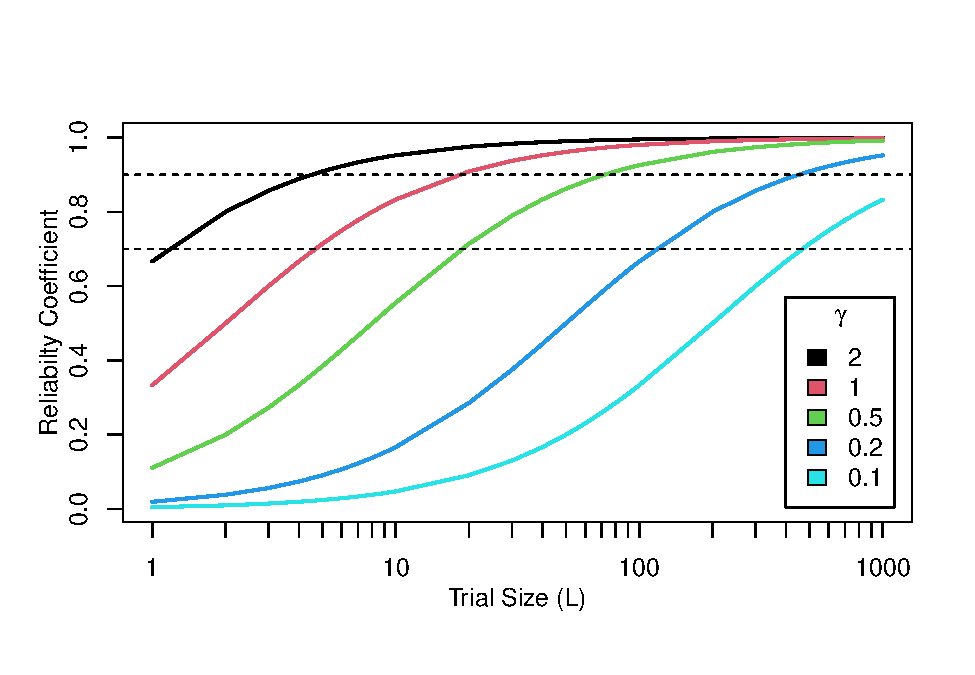
\includegraphics{p_files/figure-latex/rel-1.pdf}
\caption{\label{fig:rel}Reliability coefficients as a function of trial size for various signal-to-noise-standard-deviation ratios \(\gamma\). Horizontal lines at .7 and .9 can be used to plan the trial size for tasks with contrasts across conditions such as the Stroop task.}
\end{figure}

\hypertarget{calcuations-of-signal-to-noise-ratios}{%
\section{Calcuations of Signal-To-Noise Ratios}\label{calcuations-of-signal-to-noise-ratios}}

It is possible to derive straightforward formula for these ratios without performing any model analysis. For a single task, the sample effect, \(d_i\), is distributed as \(d_i\sim \mbox{Normal}(\nu,2\sigma^2/L+\delta^2)\). Hence, the usual sample variance has an expectation of \(\mbox{E}[\mbox{Var}(d)]=2\sigma^2/L+\delta^2\). Substituting in \(\gamma^2\) yields, \(\mbox{E}[\mbox{Var}(d)]=\sigma^2(2/L+\gamma^2)\). Rearranging yields the following estimator of \(\gamma^2\):\footnote{For tasks without contrasts, the analogous formula is \(\hat{\gamma}^2 = \frac{\mbox{Var}(d)}{\hat{\sigma}^2}-\frac{1}{L}.\)}

\begin{eq} \label{sampGammaTask}
\hat{\gamma}^2 = \frac{\mbox{Var}(d)}{\hat{\sigma}^2}-\frac{2}{L}.
\end{eq}

\(\mbox{Var}(d)\) is the sample variance, \(\sum_i (d_i-\bar{d})^2/(I-1)\), and \(\hat{\sigma}^2\) is the MSE given by \(\sum_{ijk} (Y_{ijk}-\bar{Y}_{ij})^2/(IJ(K-1))\).

\hypertarget{the-consequences-of-low-and-high-signal-to-noise-ratios}{%
\section{The Consequences of Low and High Signal-To-Noise Ratios}\label{the-consequences-of-low-and-high-signal-to-noise-ratios}}

\begin{figure}
\centering
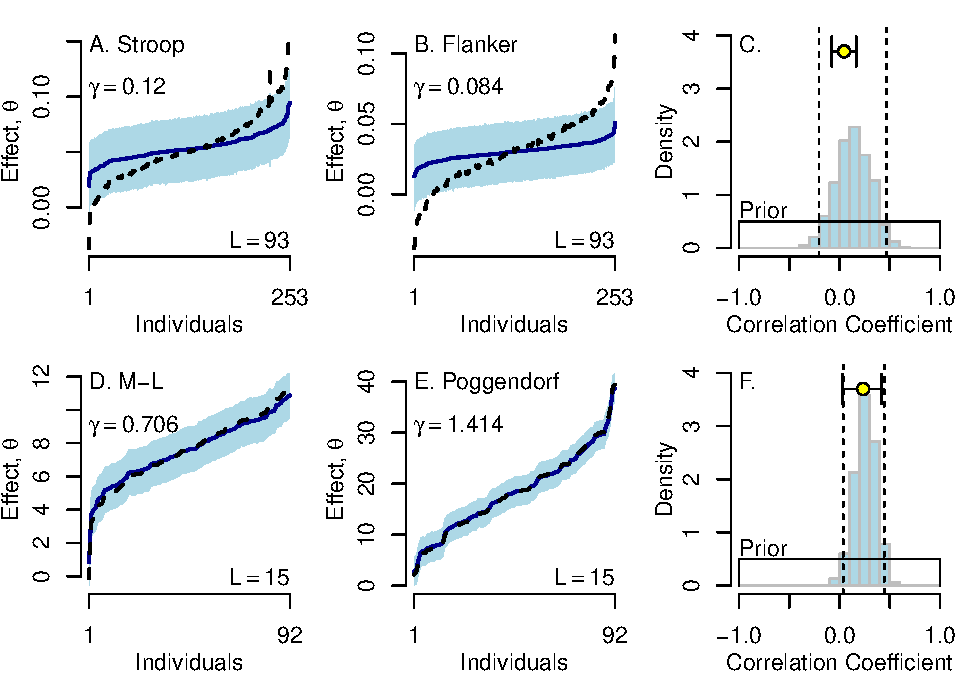
\includegraphics{p_files/figure-latex/reg-1.pdf}
\caption{\label{fig:reg}A-B. Observed effects (\(d_i\), dashed line) and model-based estimates (\(\theta_i\), solid line) for Rey Mermet et al.'s (2018) Stroop and flanker tasks. The shaded area shows the 95\% credible interval for model-based effects. The signal-to-noise ratio \(\gamma\) is low indicating much trial noise. C. Posterior distribution of model-based correlation (\(\rho\)) between Stroop and flanker effects. The dashed lines denote the 95\% credible interval. The point and segments above the distribution show the observed corrlelation coefficient and associated 95\% CI. D-E. Analogous plots for the Mueller-Lyar and Poggendorf illusions F. Anaologous plot for the correlation between Mueller-Lyar and Poggendorf effects.}
\end{figure}

To show the consequences of low and high signal-to-noise ratios, we analyze data from a cognitive-control battery and a visual-illusions battery. There are two analyses: 1. a conventional analysis in which the analysis starts from person-by-task sample effects, and observed correlations among these are the targets (see Fig. \ref{fig:usual}); and 2. a hierarchical-model analysis where trial noise is explicitly modeled.

The cognitive-control tasks come from Rey-Mermet et al. (2018), who had young and elderly participants perform a large battery. We highlight data from a number-Stroop task and a letter-flanker task. Figure \ref{fig:reg}A shows results for the Stroop task. Plotted are observed effects \(d_i\) and model estimates of \(\theta_i\). Here, the two estimators differ, and the model estimators are far more compact or regularized than the corresponding observed effects. The large degree of regularization means that the apparent individual differences in observed effects are due to trial noise and are not replicable. Fig. \ref{fig:reg}A shows the model estimate of \(\gamma\) (\(\hat{\gamma}=\)
0.12), and the number of trials (\(L=93\)). Figure \ref{fig:reg}B shows the same for the flanker task; the signal-to-noise ratio is even lower than that for the Stroop task.

Figure \ref{fig:reg}C shows the correlation among tasks. The observed correlation and associated 95\% CI is shown as a large dot and horizontal line near the top of the distribution. The correlation value is attenuated, and the relatively narrow CI reflects the large number of participants without consideration of trial noise. Comparison to the model estimates show that this high degree of confidence is misplaced. The posterior distribution of correlation from the hierarchical model is plotted along with 95\% credible intervals. The uncertainty from low signal-to-noise ratios in the tasks is reflected in the large degree of uncertainty in correlation. Of note, the observed correlation, 0.045 is attenuated by a factor of 3.06 compared to the hierarchical estimate of 0.139. In summary, low signal-to-noise ratios may result in much uncertainty when trial noise is considered and much overconfidence in heavily-attenuated values when trial noise is ignored. This summary holds for reasonably-sized samples, and the situation is not desirable.

The bottom row of Figure \ref{fig:reg} shows a more sanguine case. The data are from a pilot study on visual illusions gathered by the authors and Michael S. Pratte. The paradigm for the illusions is shown in Figure \ref{fig:ill}. For the Mueller-Lyar paradigm, participants adjusted a center arrow so that it bisects the horizontal line. Participants' tendency is to set the center arrow too far to the left, and we coded that as a positive bias. For the Poggendorf paradigm, participants adjusted the vertical offset of the right segment so that it lined up with the extension of the left segment through the occluded region. Participants' tendency is to set this segment too far down, and we coded this as a positive bias. A total of 100 individuals from Prolific ran 15 trials in each illusion; of these 100 individuals, 7 were discarded for producing uninterpretable data.

The resulting biases in perception are shown in Figure\ref{fig:reg}D-E. As can be seen, illusion tasks yield quite high signal-to-noise ratios. These high-ratios agree well with Cretenoud, Grzeczkowski, Kunchulia, and Herzog (2021), who studied individual differences in Mueller-Lyar, Ebbinghaus, and Ponzo illusions. With high signal-to-noise ratios, there is little regularization and sample mean estimates match hierarchical estimates even with the limited number of trials. Moreover, with high signal-to-noise ratios, observed and model correlations match in both value and uncertainty (Fig. \ref{fig:reg}F). In this case, because trial noise is small relative to individual variation, the uncertainty in correlation reflects the moderate number of people rather than the limited number of trials.

\begin{figure}
\centering
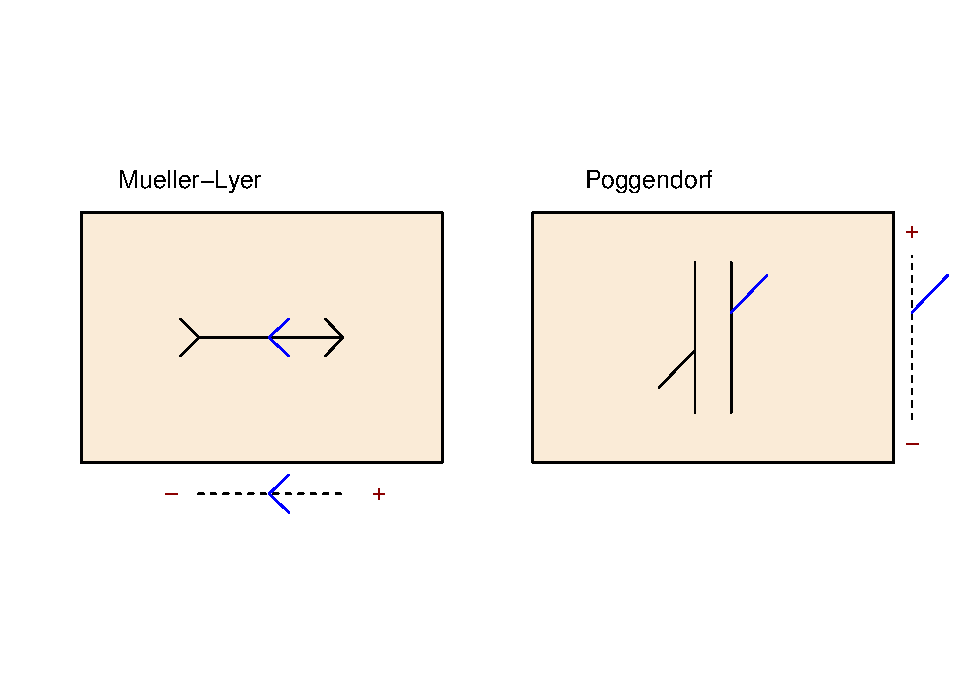
\includegraphics{p_files/figure-latex/ill-1.pdf}
\caption{\label{fig:ill}Paradigms for assessing visual illusions. Left: For the Muelller-Lyar paradigm, participants adjusted a center arrow so that it bisects the horizontal line. Right: For the Poggendorf illusion, participants adjusted the vertical offset of the right segment so that it lined up with the extension of the left segment through the occluded region.}
\end{figure}

\hypertarget{signal-to-noise-ratios-in-a-few-tasks-and-measures}{%
\section{Signal-To-Noise Ratios In A Few Tasks and Measures}\label{signal-to-noise-ratios-in-a-few-tasks-and-measures}}

The critical quantity for planning experiments and understanding the ability to localize correlations is the signal-to-noise ratio. What are the values for a range of tasks? Table \ref{tab:allTasks} provides some guidance.

\begin{table}[tbp]

\begin{center}
\begin{threeparttable}

\caption{\label{tab:allTasks}}

\begin{tabular}{lccccc}
\toprule
 & \multicolumn{1}{c}{Design} & \multicolumn{2}{c}{Signal-To-Noise SD
                        Estimates} & \multicolumn{2}{c}{Needed Trial Size} \\
\cmidrule(r){2-2} \cmidrule(r){3-4} \cmidrule(r){5-6}
Tasks & \multicolumn{1}{c}{Contrast} & \multicolumn{1}{c}{Eq} & \multicolumn{1}{c}{Model} & \multicolumn{1}{c}{r = 0.7} & \multicolumn{1}{c}{r = 0.9}\\
\midrule
Body Measure &  &  &  &  & \\
\ \ \ 1. Weight & N & 11.48 & - & 1 & 1\\
Stroop &  &  &  &  & \\
\ \ \ 2. Effect & Y & 0.12 & 0.12 & 158 & 607\\
\ \ \ 3. Speed & N & 0.96 & 0.96 & 3 & 10\\
Flanker &  &  &  &  & \\
\ \ \ 4. Effect & Y & 0.07 & 0.08 & 353 & 1359\\
\ \ \ 5. Speed & N & 0.70 & 0.7 & 5 & 19\\
Lexical Distance &  &  &  &  & \\
\ \ \ 6. Effect & Y & 0.11 & 0.11 & 193 & 742\\
\ \ \ 7. Speed & N & 0.60 & 0.62 & 7 & 24\\
Illusions &  &  &  &  & \\
\ \ \ 8. Mueller-Lyar & N & 0.72 & 0.71 & 5 & 19\\
\ \ \ 9. Poggendorf & N & 1.46 & 1.41 & 2 & 5\\
\bottomrule
\addlinespace
\end{tabular}

\begin{tablenotes}[para]
\normalsize{\textit{Note.} The standard deviation of repeated weight measurements was assumed at 3 lbs.}
\end{tablenotes}

\end{threeparttable}
\end{center}

\end{table}

The first row is for weight. We used the U.S. Army's 2012/2014 survey of 6068 soldiers' anthropometric data (Army, 2014). The mean and standard deviation of weight are 175.4 lbs and 34.4 lbs, respectively. How variable are weight measurements? Let's assume that a repeat measurements might have an standard deviation of 3 lbs. Although 3 lbs is likely too high, it is a small amount relative to the variation across participants, and \(\gamma =\) 11.48. Weight is a best-case scenario---the range of human weights compared to the reliability of scales is indeed quite large.

The next rows are for the Rey-Mermet et al.~Stroop task, and Row 2 shows the signal-to-noise ratio for the Stroop effect. The columns \texttt{Eq} and \texttt{Model} show the estimate of \(\gamma\) from Eq. \ref{sampGammaTask} and the hierarchical model, respectively. These values match well in all cases. Following that are the number of trials needed to attain a criterial level of reliability. For the Stroop effect, the signal-to-noise is low, and the needed trial sizes are large. The following row, Row 3, is for the average or overall speed rather than the contrast. Here, the signal-to-noise ratio is great, that is, the variability in participants in overall speed is large relative to trial noises. Hence, only 10s of trials per person are needed to localize individual differences in overall speed.

There is one new task, lexical distance, which is an implementation of the distance-from-five effect (Moyer \& Landauer, 1967). Participants classified digits as either less-than or greater-than five, and did so more quickly if the digit was far from five (digits 2 and 8) than close to five (digits 4 and 6). The contrast row is for the contrast between near and far digits; the speed row is for the overall speed. As with cognitive-control tasks, the signal-to-noise is much greater for localizing individual overall speed effects than for localizing individual distance-from-five effects.

\hypertarget{the-reliability-crisis-revisited}{%
\section{The Reliability Crisis Revisited}\label{the-reliability-crisis-revisited}}

The reliability of a task can be profitably assessed without recourse to trial size when reliability is a signal-to-noise ratio. With it, researchers can communicate clearly about reliability without recourse to trial size. Signal-to-noise ratios succinctly capture how well individual differences may be localized and how well the structure of covariation of individual differences across tasks may be recovered. Moreover, the ratio may be estimated accurately from common sample variances without modeling. The simple formulas provided here may be used for planning an experiment or for interpreting whether small correlations reflect a true lack of correlation or attenuation from low reliability. The advantage of hierarchical-model analysis is the resultant measures of uncertainty on correlations across tasks.

The cause of the reliability crisis is that researchers tend to use too few trials in tasks with too low signal-to-noise ratios. One obvious solution is to use more trials. For example, the correlation between Stroop and flanker can be well localized with \(L=500\) trials per person per condition. The problem with this obvious solution is that increasing the trial size is often unrealistic or inconvenient. Some of the drawbacks to great numbers of trials are that fewer tasks may be run in a battery, effects may attenuate with practice, and people may fatigue or even withdraw.

There are other proposed solutions to the reliability crisis that are not as draconian as implementing excessive trial sizes. These include avoiding difference scores (Draheim, Mashburn, Martin, \& Engle, 2019), using so-called gamified tasks (Deveau, Jaeggi, Zordan, Phung, \& Seitz, 2015; Kucina et al., 2022), and diffusion modeling (Haines et al., 2020; Lerche et al., 2020; von Krause, Lerche, Schubert, \& Voss, 2020; Weigard, Clark, \& Sripada, 2021). Understanding the concept of signal-to-noise helps to evaluate these proposals (e.g., Kucina et al., 2022).

Our preference is to avoid tasks with low signal-to-noise ratios because the recovery of covariation is so precarious. High signal instruments include overall speed and biases in visual illusions. We advocate a prioritization of high-signal instruments even at the expense of more traditional albeit low-signal instruments (see Draheim, Tsukahara, Martin, Mashburn, \& Engle, 2021 for a related view). Even without these low-signal instruments, there is a rich cognitive world that may be explored fruitfully with individual differences. For example, what is the factor structure of overall speed across a wide range of tasks? Is there a single susceptibility-to-visual-illusions factor? We hope the development facilitates this fruitful exploration.

\newpage

\hypertarget{references}{%
\section*{References}\label{references}}
\addcontentsline{toc}{section}{References}

\hypertarget{refs}{}
\begin{CSLReferences}{1}{0}
\leavevmode\vadjust pre{\hypertarget{ref-Army.2014}{}}%
Army. (2014). \emph{2012 {Anthropometric Survey} of {U}.{S}. {Army Personnel}: {Methods} and {Summary Statistics}} (No. ADA611869). {Army Natick Soldier Research and Engineering Center}. Retrieved from \url{https://apps.dtic.mil/sti/citations/ADA611869}

\leavevmode\vadjust pre{\hypertarget{ref-Bollen.1989}{}}%
Bollen, K. A. (1989). \emph{Structural equations with latent variables}. {Wiley}.

\leavevmode\vadjust pre{\hypertarget{ref-Cretenoud.etal.2021}{}}%
Cretenoud, A. F., Grzeczkowski, L., Kunchulia, M., \& Herzog, M. H. (2021). Individual differences in the perception of visual illusions are stable across eyes, time, and measurement methods. \emph{Journal of Vision}, \emph{21}(5), 26--26.

\leavevmode\vadjust pre{\hypertarget{ref-Deveau.etal.2015}{}}%
Deveau, J., Jaeggi, S. M., Zordan, V., Phung, C., \& Seitz, A. R. (2015). How to build better memory training games. \emph{Frontiers in Systems Neuroscience}, \emph{8}, 243.

\leavevmode\vadjust pre{\hypertarget{ref-Draheim.etal.2019}{}}%
Draheim, C., Mashburn, C. A., Martin, J. D., \& Engle, R. W. (2019). Reaction time in differential and developmental research: {A} review and commentary on the problems and alternatives. \emph{Psychological Bulletin}, \emph{145}(5), 508.

\leavevmode\vadjust pre{\hypertarget{ref-Draheim.etal.2021}{}}%
Draheim, C., Tsukahara, J. S., Martin, J. D., Mashburn, C. A., \& Engle, R. W. (2021). A toolbox approach to improving the measurement of attention control. \emph{Journal of Experimental Psychology: General}, \emph{150}(2), 242.

\leavevmode\vadjust pre{\hypertarget{ref-Enkavi.etal.2019}{}}%
Enkavi, A. Z., Eisenberg, I. W., Bissett, P. G., Mazza, G. L., MacKinnon, D. P., Marsch, L. A., \& Poldrack, R. A. (2019). Large-scale analysis of test--retest reliabilities of self-regulation measures. \emph{Proceedings of the National Academy of Sciences}, \emph{116}(12), 5472--5477.

\leavevmode\vadjust pre{\hypertarget{ref-Eriksen.Eriksen.1974}{}}%
Eriksen, B. A., \& Eriksen, C. W. (1974). Effects of noise letters upon the identification of a target letter in a nonsearch task. \emph{Perception \& Psychophysics}, \emph{16}, 143--149.

\leavevmode\vadjust pre{\hypertarget{ref-Haines.etal.2020}{}}%
Haines, N., Kvam, P. D., Irving, L. H., Smith, C., Beauchaine, T. P., Pitt, M. A., \ldots{} Turner, B. M. (2020). Theoretically informed generative models can advance the psychological and brain sciences: {Lessons} from the reliability paradox.

\leavevmode\vadjust pre{\hypertarget{ref-Hedge.etal.2018}{}}%
Hedge, C., Powell, G., \& Sumner, P. (2018). The reliability paradox: {Why} robust cognitive tasks do not produce reliable individual differences. \emph{Behavioral Research Methods}.

\leavevmode\vadjust pre{\hypertarget{ref-Kane.etal.2001}{}}%
Kane, M. J., Bleckley, M. K., Conway, A. R. A., \& Engle, R. W. (2001). A controlled-attention view of working-memory capacity. \emph{Journal of Experimental Psychology: General}, \emph{130}(2), 169--183. Retrieved from \url{http://search.ebscohost.com/login.aspx?direct=true\&db=psyh\&AN=2001-17501-002\&loginpage=Login.asp\&site=ehost-live\&scope=site}

\leavevmode\vadjust pre{\hypertarget{ref-Karr.etal.2018}{}}%
Karr, J. E., Areshenkoff, C. N., Rast, P., Hofer, S. M., Iverson, G. L., \& Garcia-Barrera, M. A. (2018). The unity and diversity of executive functions: {A} systematic review and re-analysis of latent variable studies. \emph{Psychological Bulletin}, \emph{144}(11), 1147.

\leavevmode\vadjust pre{\hypertarget{ref-Kucina.etal.2022}{}}%
Kucina, T., Wells, L., Lewis, I., de Salas, K., Kohl, A., Palmer, M., \ldots{} Heathcote, A. (2022). A solution to the reliability paradox for decision-conflict tasks.

\leavevmode\vadjust pre{\hypertarget{ref-Lerche.etal.2020}{}}%
Lerche, V., von Krause, M., Voss, A., Frischkorn, G. T., Schubert, A.-L., \& Hagemann, D. (2020). Diffusion modeling and intelligence: {Drift} rates show both domain-general and domain-specific relations with intelligence. \emph{Journal of Experimental Psychology: General}, \emph{149}, 2207--2249. doi:\href{https://doi.org/10.1037/xge0000774}{10.1037/xge0000774}

\leavevmode\vadjust pre{\hypertarget{ref-Matzke.etal.2017}{}}%
Matzke, D., Ly, A., Selker, R., Weeda, W. D., Scheibehenne, B., Lee, M. D., \& Wagenmakers, E.-J. (2017). Bayesian inference for correlations in the presence of measurement error and estimation uncertainty. \emph{Collabra: Psychology}, \emph{3}(1).

\leavevmode\vadjust pre{\hypertarget{ref-Miyake.etal.2000}{}}%
Miyake, A., Friedman, N. P., Emerson, M. J., Witzki, A. H., Howerter, A., \& Wager, T. D. (2000). The unity and diversity of executive functions and their contributions to complex {``frontal lobe''} tasks: {A} latent variable analysis. \emph{Cognitive Psychology}, \emph{41}(1), 49--100.

\leavevmode\vadjust pre{\hypertarget{ref-Moyer.Landauer.1967}{}}%
Moyer, R. S., \& Landauer, T. K. (1967). Time required for judgements of numerical inequality. \emph{Nature}, \emph{215}, 1519--1520.

\leavevmode\vadjust pre{\hypertarget{ref-Rey-Mermet.etal.2018}{}}%
Rey-Mermet, A., Gade, M., \& Oberauer, K. (2018). Should {We Stop Thinking About Inhibition}? {Searching} for {Individual} and {Age Differences} in {Inhibition Ability}. \emph{Journal of Experimental Psychology: Learning, Memory, and Cognition}. Retrieved from \url{http://dx.doi.org/10.1037/xlm0000450}

\leavevmode\vadjust pre{\hypertarget{ref-Rouder.Haaf.2019}{}}%
Rouder, J. N., \& Haaf, J. M. (2019). A psychometrics of individual differences in experimental tasks. \emph{Psychonomic Bulletin and Review}, \emph{26}(2), 452--467. Retrieved from \url{https://doi.org/10.3758/s13423-018-1558-y}

\leavevmode\vadjust pre{\hypertarget{ref-Rouder.etal.inpreparation}{}}%
Rouder, J. N., Haaf, J. M., \& Kumar, A. (in preparationin preparation). \emph{Why {Most Studies} of {Individual Differences With Cognitive Tasks Are Bound To Fail}}.

\leavevmode\vadjust pre{\hypertarget{ref-Schubert.etal.2017}{}}%
Schubert, A.-L., Hagemann, D., \& Frischkorn, G. T. (2017). Is general intelligence little more than the speed of higher-order processing? \emph{Journal of Experimental Psychology: General}, \emph{146}(10), 1498.

\leavevmode\vadjust pre{\hypertarget{ref-Skrondal.Rabe-Hesketh.2004}{}}%
Skrondal, A., \& Rabe-Hesketh, S. (2004). \emph{Generalized {Latent Variable Modeling}: Multilevel, longitudinal, and structural equation models}. {Boca Raton}: {CRC Press}.

\leavevmode\vadjust pre{\hypertarget{ref-Spearman.1904a}{}}%
Spearman, C. (1904). The {Proof} and {Measurement} of {Association} between {Two Things}. \emph{American Journal of Psychology}, \emph{15}, 72--101. Retrieved from \url{https://www.jstor.org/stable/pdf/1412159.pdf}

\leavevmode\vadjust pre{\hypertarget{ref-Stroop.1935}{}}%
Stroop, J. R. (1935). Studies of interference in serial verbal reactions. \emph{Journal of Experimental Psychology}, \emph{18}, 643--662.

\leavevmode\vadjust pre{\hypertarget{ref-vonKrause.etal.2020}{}}%
von Krause, M., Lerche, V., Schubert, A.-L., \& Voss, A. (2020). Do {Non-Decision Times Mediate} the {Association} between {Age} and {Intelligence} across {Different Content} and {Process Domains}? \emph{Journal of Intelligence}, \emph{8}(3, 3), 33. doi:\href{https://doi.org/10.3390/jintelligence8030033}{10.3390/jintelligence8030033}

\leavevmode\vadjust pre{\hypertarget{ref-Weigard.etal.2021}{}}%
Weigard, A., Clark, D. A., \& Sripada, C. (2021). Cognitive efficiency beats top-down control as a reliable individual difference dimension relevant to self-control. \emph{Cognition}, \emph{215}, 104818. doi:\href{https://doi.org/10.1016/j.cognition.2021.104818}{10.1016/j.cognition.2021.104818}

\end{CSLReferences}


\end{document}
